\chapter{View and Feature Combination Investigations}\label{ch:view-comb}
This chapter I will be:
\begin{itemize}
  \item Creating more complicated toy tasks in RLBench
  \item Propose various imitation learning agents to solve these tasks
  \item Evaluate said methods by:
  \begin{enumerate}
    \item Providing different views and features
    \item Augmenting the fusion of these features
    \item Understand how the agent `views' a scene and what information it benefits from for which tasks
    \item Compare the strengths and weaknesses of these methods
  \end{enumerate}
\end{itemize}

% Reaching (NoObs) tasks
\section{Experimenting with Reaching}\label{sec:reach-no-obs}

\subsection{Creating a Policy}
The next step was to create a policy network. As I am mainly working on imitation learning -and specifically behavioural cloning- from demonstrations provided by the system. A network needs to be able to ingest these demonstrations and generate actions in the action space of the robot. Following the earlier parameters of a demo, I created the following network, Figure \ref{fig:policy-arch}. This takes in the given wrist rgb image and extracts features, which are then interpreted into a $8$ dim vector of \textbf{float}s as an action of joint velocities. First $7$ corresponding to the $7$ joints of the \emph{Panda} robot, while the final value is the gripper state, $0$ meaning closed and $1$ meaning open, which is clamped by the movement system under the hood.

\begin{figure}[h]
  \centering
  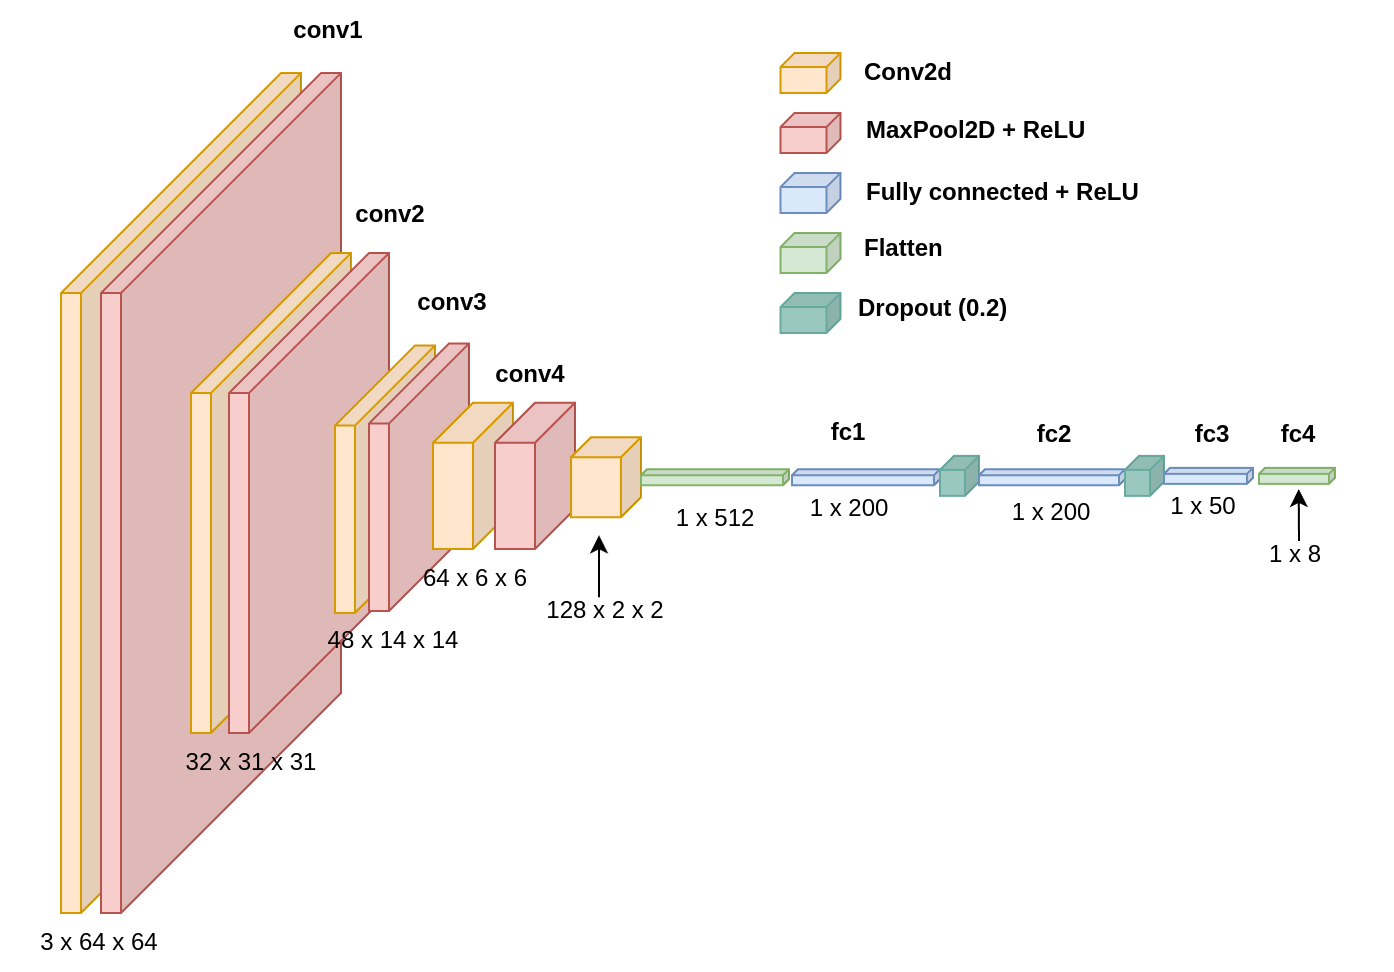
\includegraphics[width=0.4\textwidth]{assets/early-work/cnn-encoder-policy-head.png}
  \caption{Simple Policy Network Architecture}\label{fig:policy-arch}
\end{figure}\todo[color=blue]{ius the quality bad? reuload or reexport the xmml is in assets}


\subsubsection{Data Processing}\todo[color=red]{talk about rgb transforms? uniforming etc, or not not sure}
How the data is regularised, processed, and loaded into the system for training or testing is quite important for any Machine Learning (ML) task. The main processing I applied to the data was normalisation and scaling. RLBench, by default, returns image colour values in the range \(\left[0, 255\right]\) which was transformed to be in range \(\left[0.0, 1.0\right]\). Done before both inference and training. Mainly to keep weight magnitudes manageable for faster convergence, due to optimisers and activation functions working better at smaller scales. Secondly, this means that each pixel in the image will contribute to the extruded feature proportionally. Without the use of raw, meaningless numbers. This will help the numerical stability of the task.

\subsubsection{Data Loading}\label{subsec:reach-data-loading}
I followed a simple flattening approach for loading the data into the system. Using PyTorch's \textbf{Dataset} and \textbf{DataLoader} classes I created a dataset that can take in a raw list of demonstration, then flattens its observations into a tensor of shape \(\langle 3,~64,~64 \rangle \) (permuted from the usual \(\langle 64,~64,~3 \rangle \) for images due to Torch conventions of convolutional networks and where they expect the channel  dimension). Then the dataset makes individual observation indexable along with their corresponding action labels. Types given as:\mintinline{python}|DemoObsDataset: tuple[tensor[3,  64, 64], tensor[8]]|. Then the loader can manage the shuffling and batching as usual. Initially I kept the data unshuffled, to keep the data in its sequential form. While keeping the batch size as the demo length. This is because currently I am trying to overfit the network to the single demonstration given to it to gauge how long to train my networks for

\subsection{Initial Observations}
Starting with the 3 static versions of the task, where the target is placed as shown in \ref{fig:no-obs-3-views} seen from the wrist cameras. I wanted to get an idea of how to tune the policy parameters. While understanding the relationship between training length and varying observability of the target.

\begin{figure}[htbp]
  \begin{subfigure}{0.3\linewidth}
    \centering
    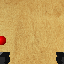
\includegraphics[width=0.6\linewidth]{assets/cam-comb/reach-no-obs/initial-obs-side_l.png}      
    \caption{Left Side}
  \end{subfigure}
  \hfill
  \begin{subfigure}{0.3\textwidth}
    \centering
    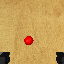
\includegraphics[width=0.6\linewidth]{assets/cam-comb/reach-no-obs/initial-obs-central.png}
    \caption{Central}
  \end{subfigure}
  \hfill
  \begin{subfigure}{0.3\textwidth}
    \centering 
    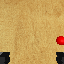
\includegraphics[width=0.6\linewidth]{assets/cam-comb/reach-no-obs/initial-obs-side_r.png}
    \caption{Right Side}
  \end{subfigure}%
  \caption{Three variations of the reach task with the obstacles sometimes out of view}\label{fig:no-obs-3-views}
\end{figure}

I tested multiple epochs of training with the simple policy and recorded the final distance to the target at the end of their episode. The episode length is determined by the demo lengths, which I defaulted to the maximum, will also try mean, as keeping a static episode length doesn't make sense (especially on later tasks where the demonstration episodes can drastically vary in length)

The success of the tasks are wired to reaching the target in the simulator and will send a \emph{DONE} signal if it is reached. This happens around $0.12$ metres to the target. I have also observed the target will reach a very close distance but it won't trigger the detection in Coppelia, I think this must be a bounding box issue, wither the dummy objects that are doing the collision detection are missing each other, or the polling rate in the simulator is not frequent enough to detect this change. Either way, I added a way to count closeness into success if it were close enough.

\subsubsection{Static Tasks}
Testing on the static versions of the task, a simple policy with training around $20$ to $100$ epochs seems to do the job well, see Figure \ref{fig:rno-static}. And this is mostly because without variation in position simple Behavioural Cloning can be employed by overfitting to the data given. 

As I trained for longer it seemed to overfit early move really slowly at the start of the episode, wasting steps and ending up far from the target. Curious observation is \todo[color=purple]{} the central tasks behaves better at higher epochs which I believe is not necessarily because of visibility (the \emph{conv} features are not necessarily guiding anything with $1$ demo) but rather the centrality, as it is right above the gripper a simple downward bias allows the arm to easily get close to the target.

\begin{figure}[htpb] % htpb allows all placement
  \centering
  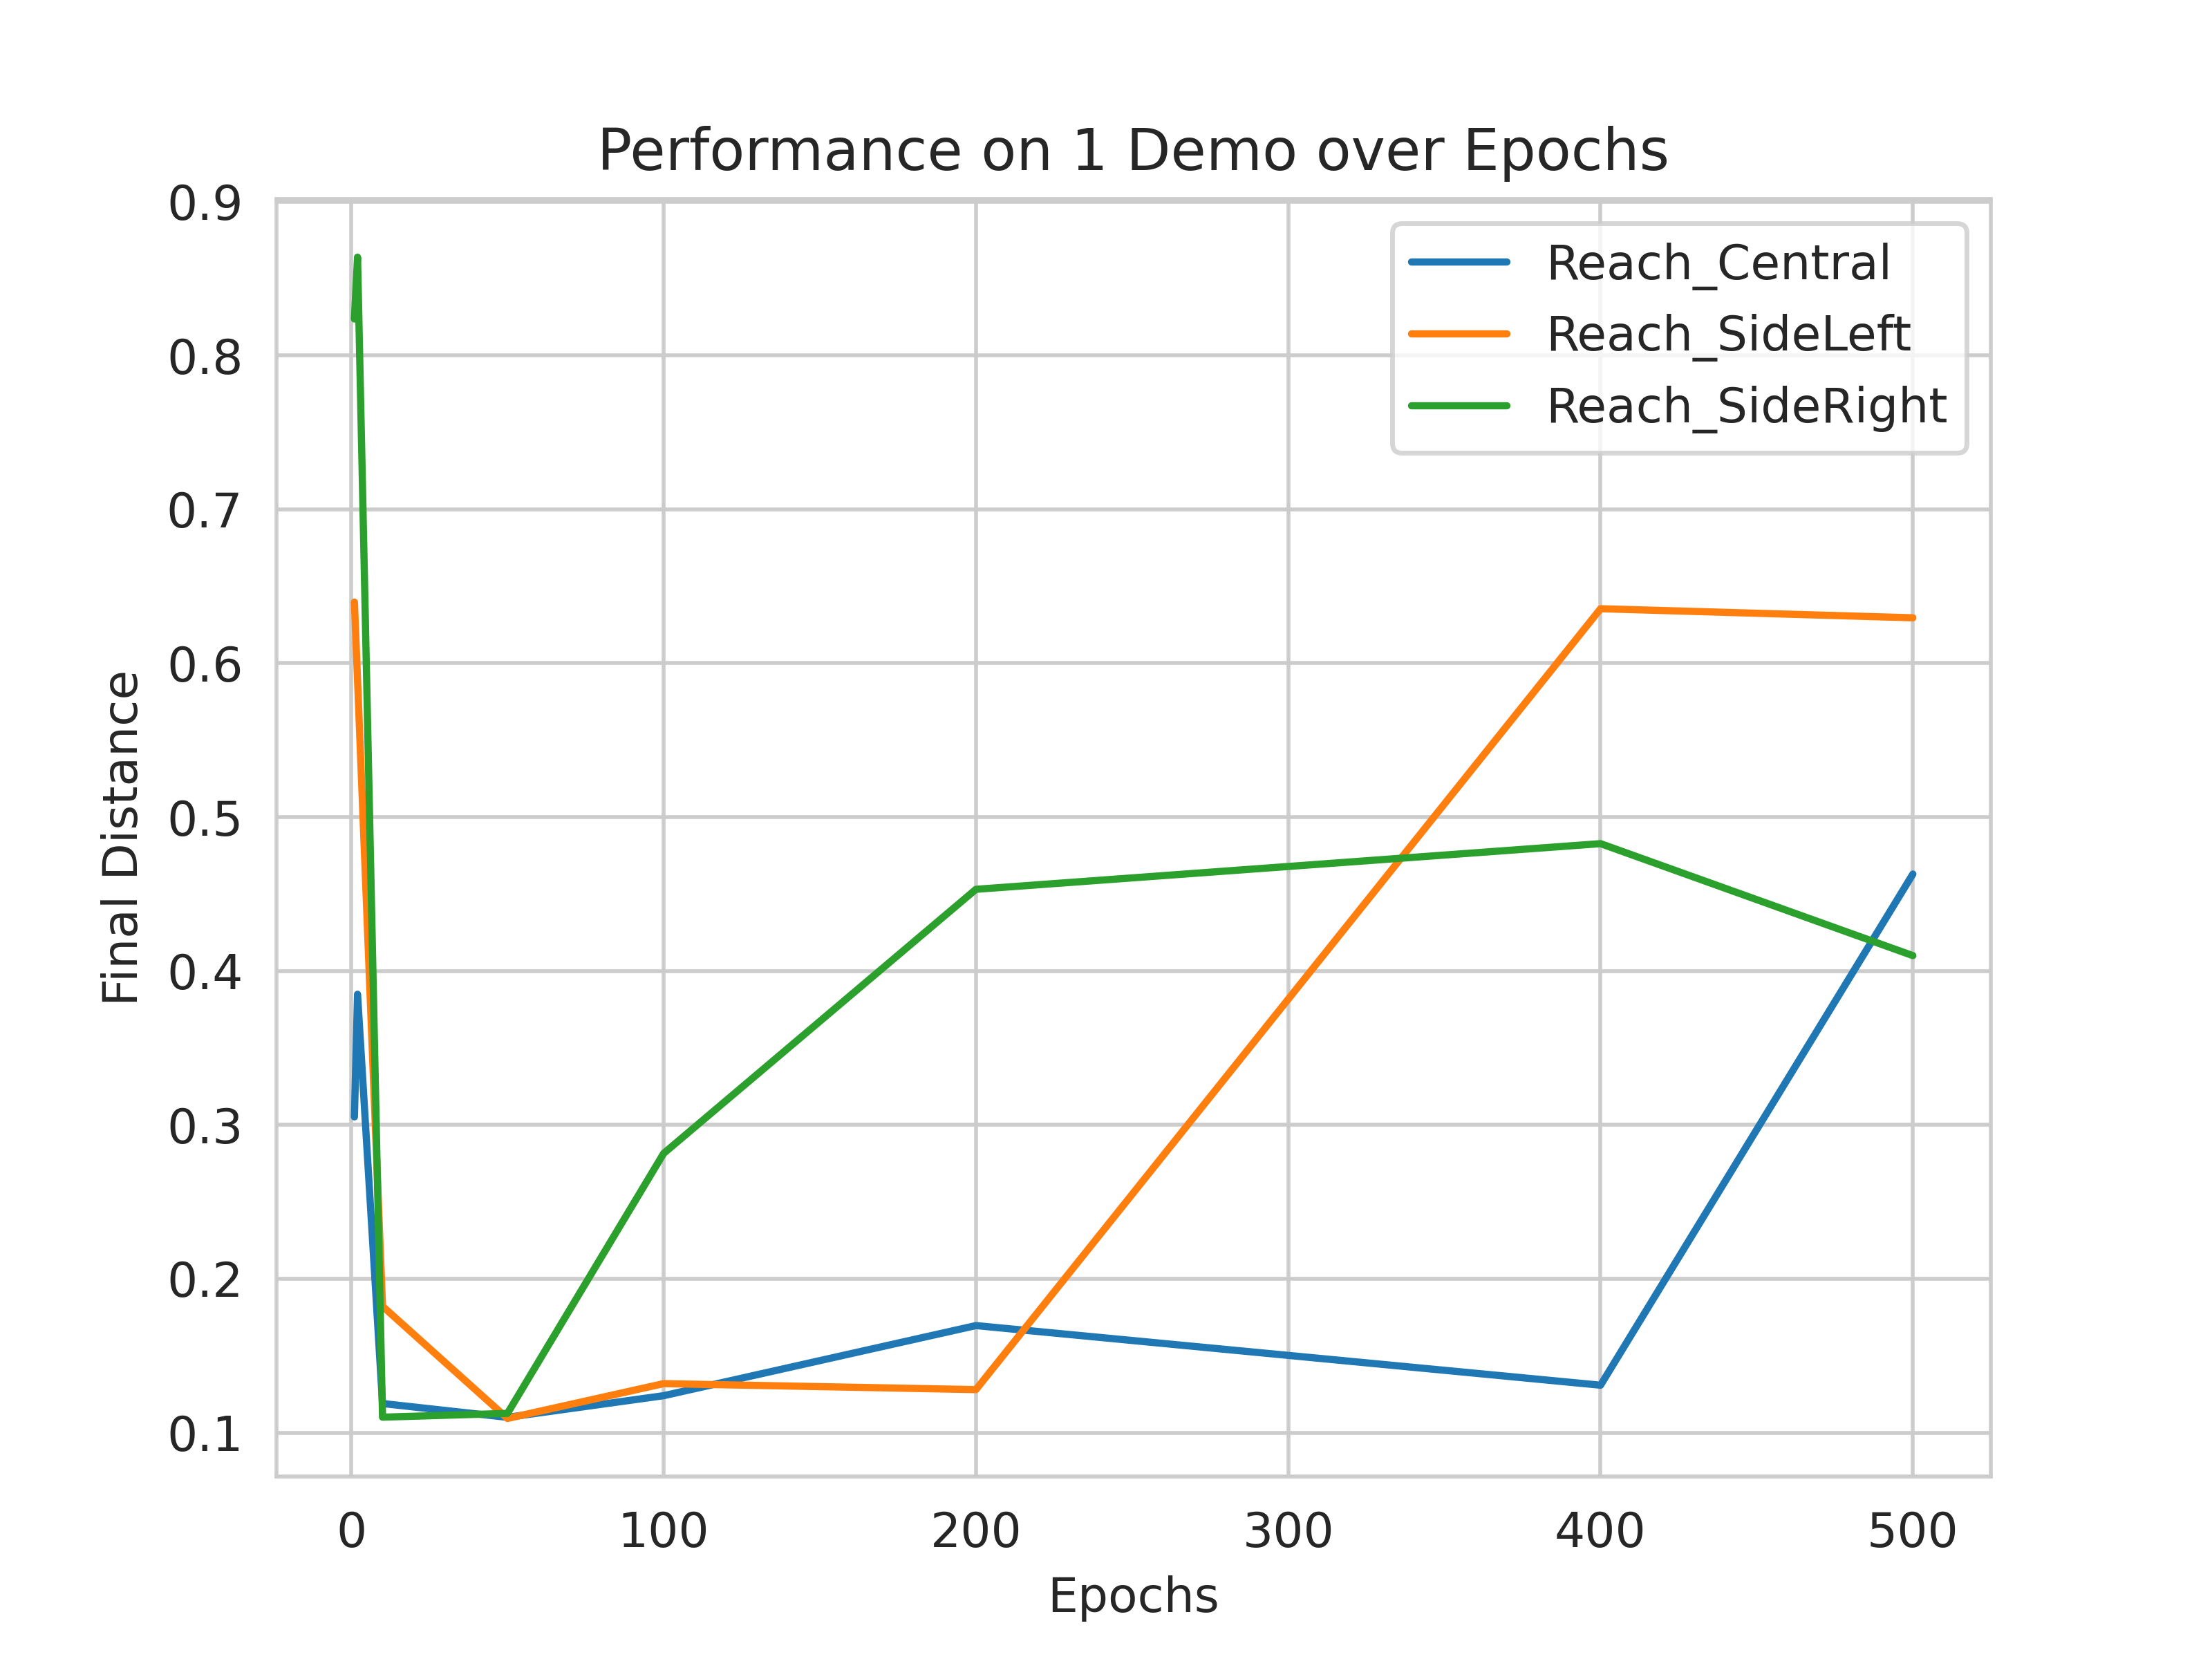
\includegraphics[scale=0.5]{assets/cam-comb/reach-no-obs/rno_static.png}
  \caption{Epoch experiments with the static tasks using a single demonstration}\label{fig:rno-static}
\end{figure}

\subsubsection{Placing Randomly}
To test generalisability, I created a dynamic version of the task, where the target is now randomly placed within view (not necessarily always fully within view, but at least some parts are visible). This is achieved by using a \textbf{SpawnBoundary|}and randomly sampling the location of the target withing this for every new variation of the task, or for every new episode. Which can be seen in Figure \ref{fig:reach-no-obs}, the white dotted box being the boundary. This boundary is not rendered in the simulation visually. This guarantees variety in demonstrations as well as helps us create a generalisable policy.

\begin{figure}[htpb] % htpb allows all placement
  \begin{subfigure}{0.50\linewidth}
    \centering
    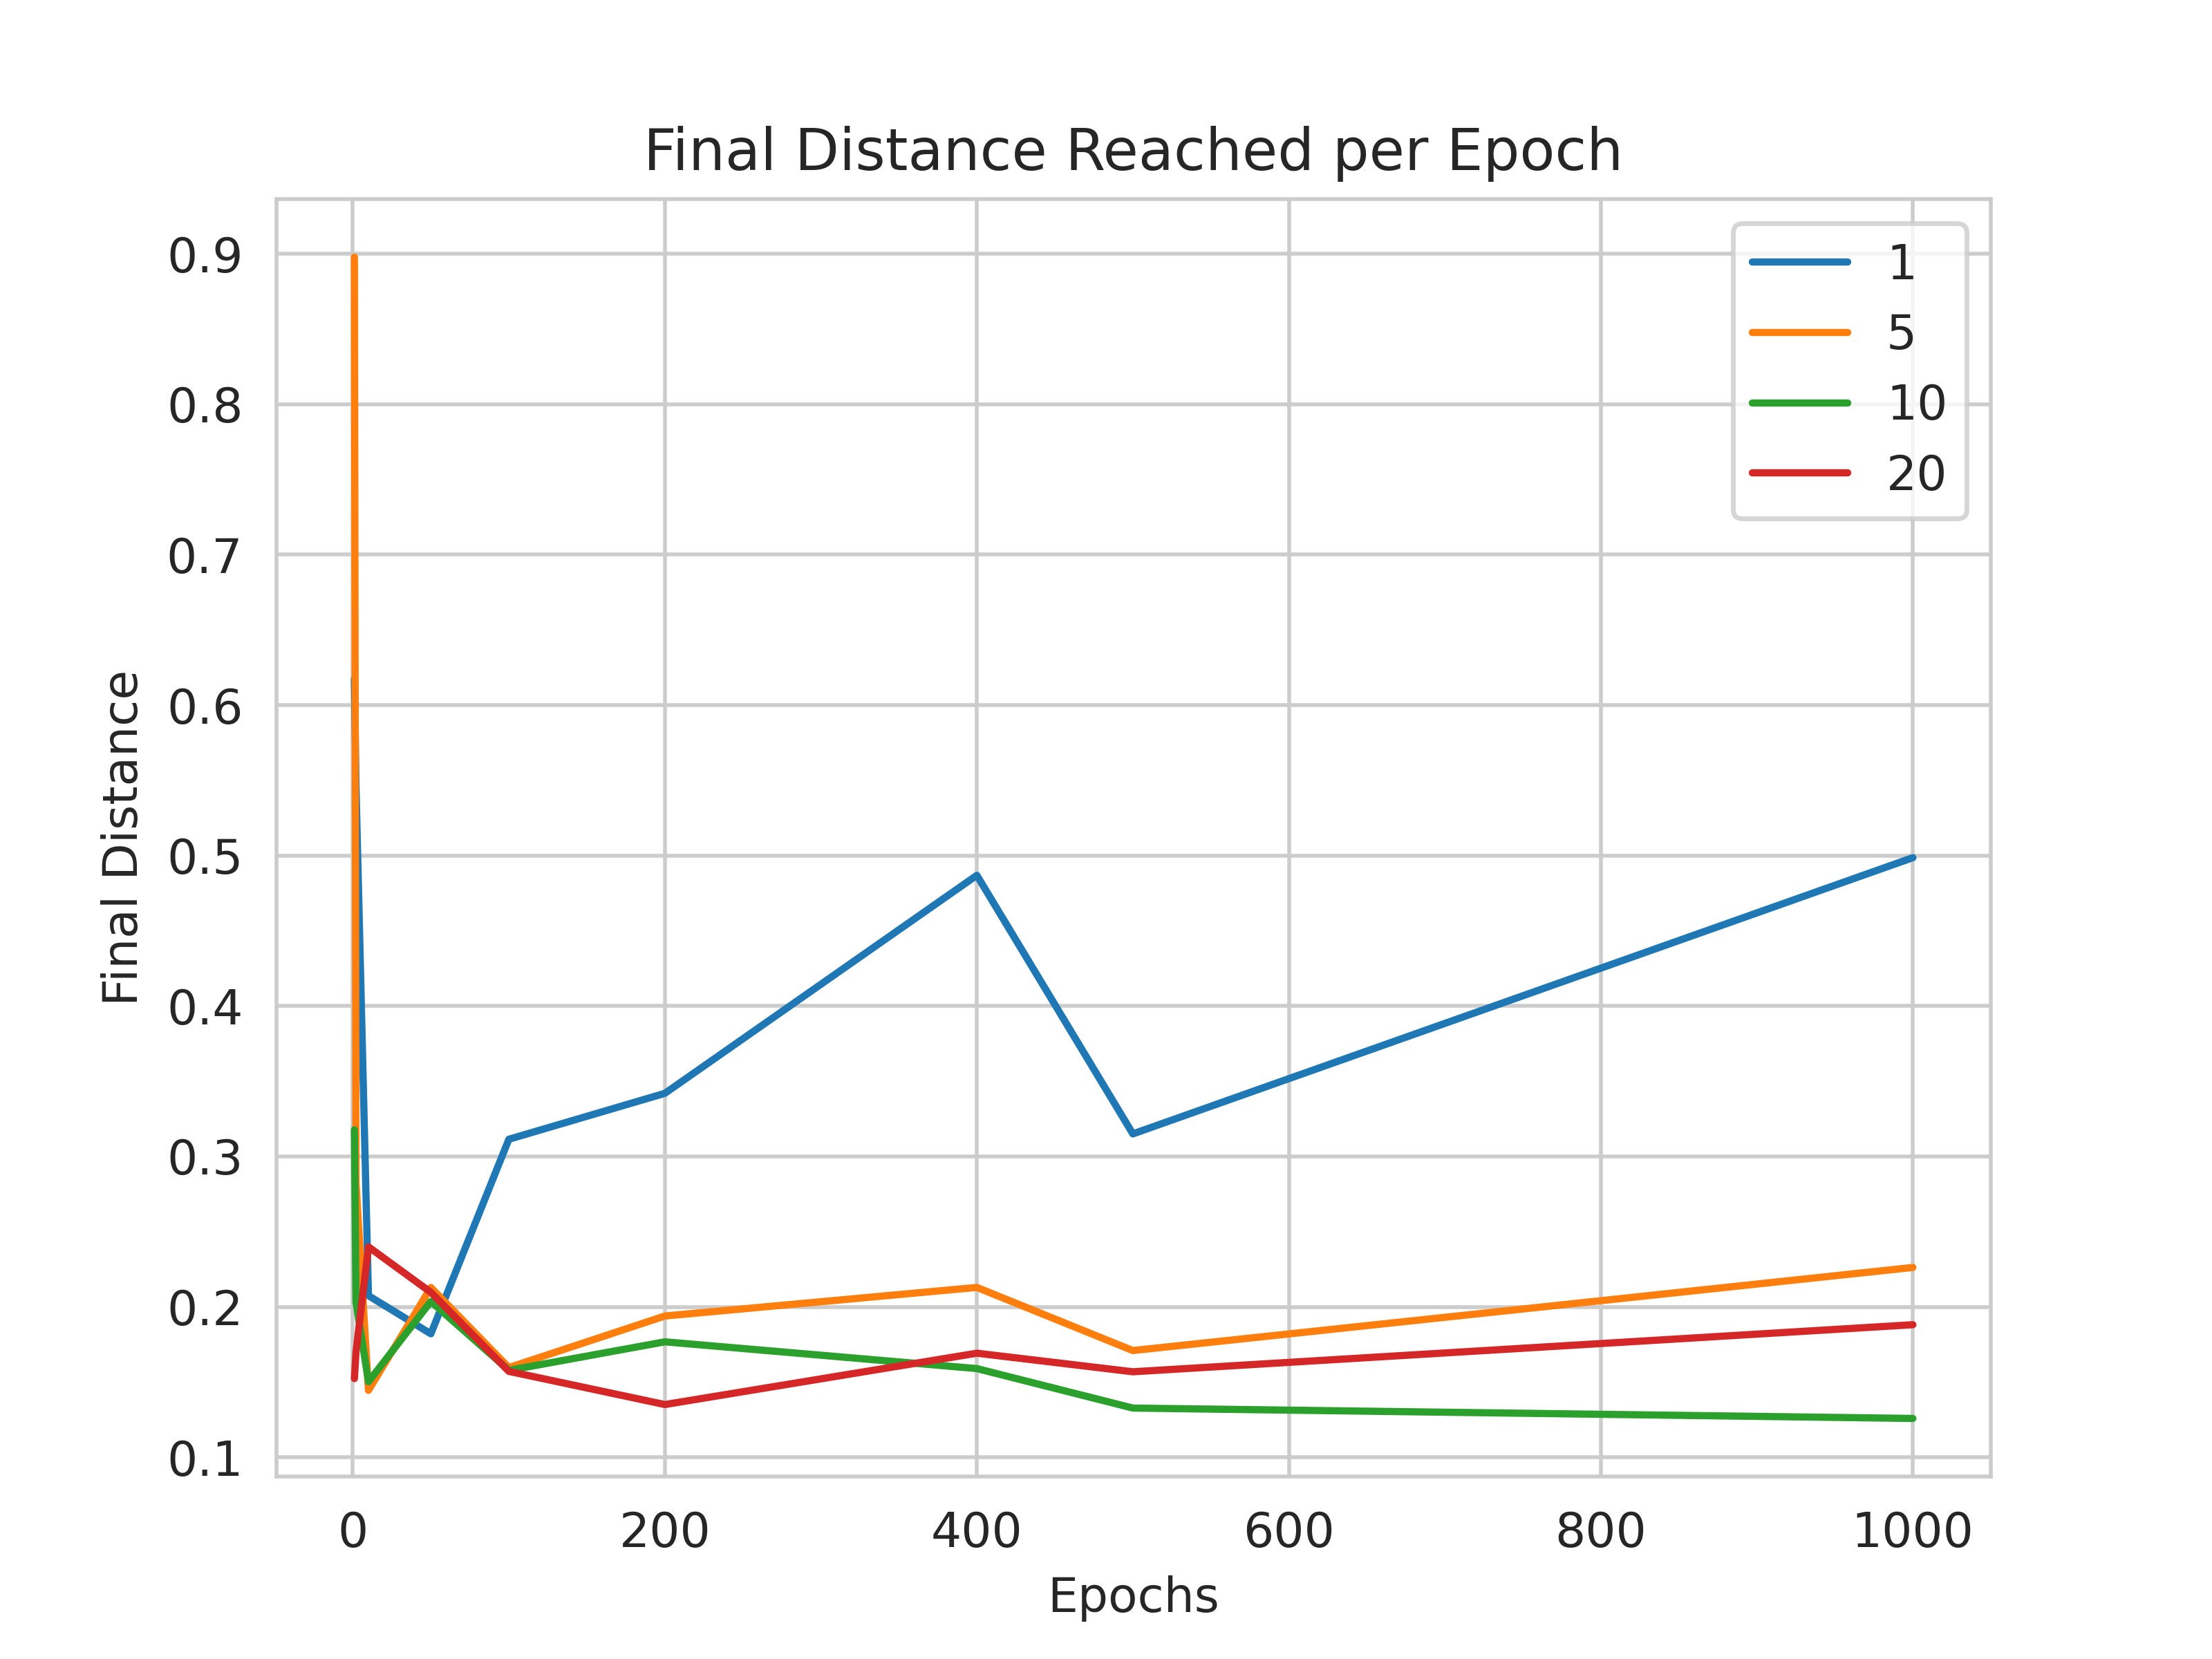
\includegraphics[width=\linewidth]{assets/cam-comb/reach-no-obs/rno_random-dist.png}
    \caption{Average Final Distance to Target}\label{subfig:rno-random-dist}
  \end{subfigure}
  \hfill
  \begin{subfigure}{0.50\linewidth}
    \centering
    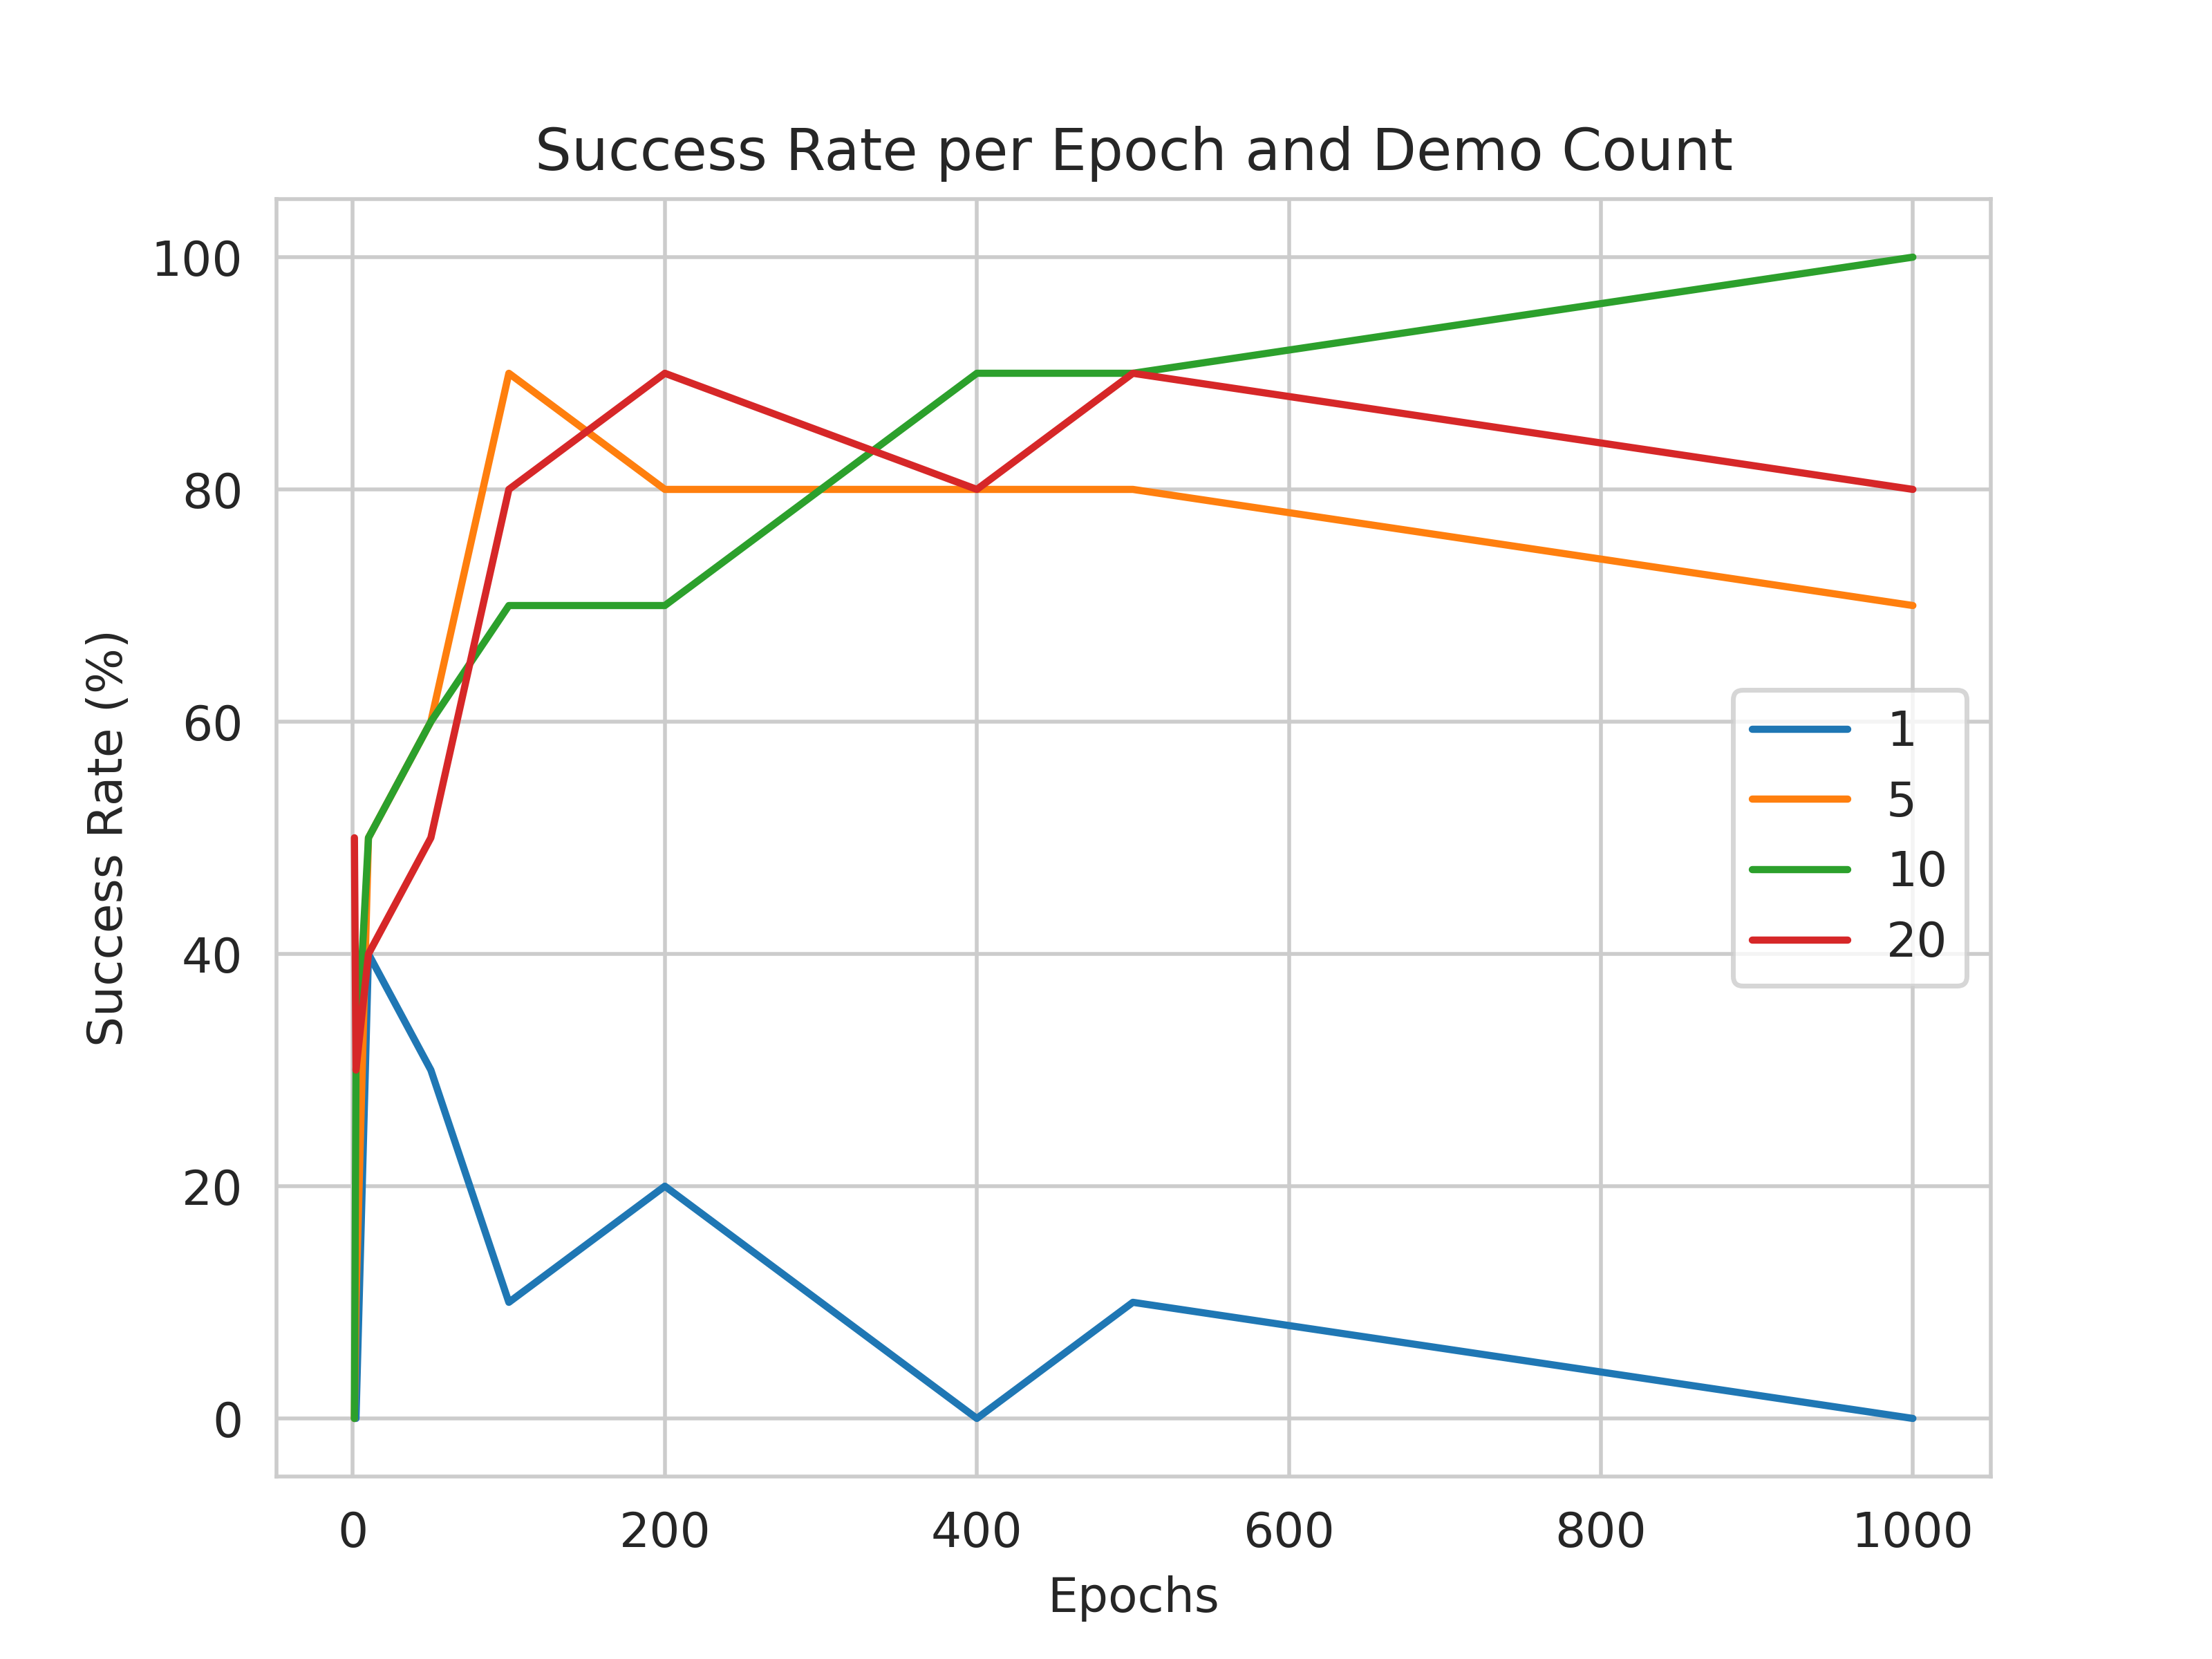
\includegraphics[width=\linewidth]{assets/cam-comb/reach-no-obs/rno_random-success.png}
    \caption{Success Rate (\%) for the $10$ Test Demos}\label{subfig:rno-random-success}
  \end{subfigure}
  \caption{Experiments with randomly placed target}\label{fig:rno-random}
\end{figure}

To run the random tests, shown in Figure \ref{fig:rno-random}, in a comparable manner I reused my set of demos that were created and saved earlier for this task for training. Then a set of 10 demos were randomly generated at the start and after the agent with the specific parameters were trained, I evaluated these policies against the test counterparts.

Looking at graph \ref{subfig:rno-random-dist}, we can see that providing more demonstrations helps the policy generalise better to random locations, where the sweet spots seems to be around 10 demos and around $500$ where the success rate (\ref{subfig:rno-random-success}) is quite high

\subsection{Camera Limitations}
I started this section by limiting the learning to only the wrist mounted camera, which works well for this specific unobscured task. Introducing some of the other RGB cameras, specifically the \textbf{left shoulder} or the \textbf{right shoulder} views, doesn't drastically benefit the performance, other than just the \textbf{right shoulder} RGB, see \ref{fig:rno-random-cams}. Conversely, combining more than one camera seems to be adding to the deficit, as the features being extracted are likely incompatible due to the various view points. 

As the current fusion system does not allow for optimal multi-view feature extraction, using multiple different cameras are not necessarily benefiting the learning and might even be negating its effectiveness due to diluting the features by concatenating incompatible views. \todo[color=green]{ref back to this when needed and improve the policy from now on?} 

A possible explanation as to why the right shoulder camera alone might be increasing success rate is, I think, solely because of its strategic placement compared to the rest of the cameras. 

It is marginally better than wrist, which is likely due to the wrist sometimes observing very similar frames if it happens to initially move away from the target, which can happen when the random target spawn location is out of distribution. Which gets the agent stuck in an unknown state in by these initial erroneous moves. Leading it to not reaching the target. This is not as big an issue with the right shoulder camera, simply due to its larger coverage, and static nature which increases the network potency in repetitive simple movements simply due to the frame of reference never changing.\todo[color=purple]{}. 

To reason why the right shoulder and not the left is simply because of the geometry of the robot. The left camera is more likely to get obstructed by the robot itself due to its top joints being on its left, seen in \ref{subfig:rno-random-ls}. 

So, there is improvement from multiple views, but this task does not really benefit from extra frames of vision. However, this is not to say all tasks will be immune to benefits from extra views. An important part of this project is to understand what is most important for a robot to observe in its given environment and task and how can it optimally leverage this data to solve a task better. And increasingly more complex tasks should benefit from abundance of information.

\begin{figure}[htpb] % htpb allows all placement
  \centering
  \begin{subfigure}{0.3\linewidth}
    \centering
    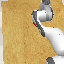
\includegraphics[width=0.8\linewidth]{assets/cam-comb/reach-no-obs/demo1-step30-left_shoulder.png}
    \caption{Left Shoulder}\label{subfig:rno-random-ls}
  \end{subfigure}
  \begin{subfigure}{0.3\linewidth}
    \centering
    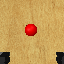
\includegraphics[width=0.8\linewidth]{assets/cam-comb/reach-no-obs/demo1-step30-wrist.png}
    \caption{Wrist}\label{subfig:rno-random-wrist}
  \end{subfigure}
  \begin{subfigure}{0.3\linewidth}
    \centering
    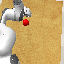
\includegraphics[width=0.8\linewidth]{assets/cam-comb/reach-no-obs/demo1-step30-right_shoulder.png}
    \caption{Right Shoulder}\label{subfig:rno-random-rs}
  \end{subfigure}
  \caption{RGB Views from the first `ReachNoObs\_PlaceRandom' demo (step 30)}\label{fig:rno-random-rgb-views}
\end{figure}

\begin{figure}[htpb] % htpb allows all placement
  \centering
  \begin{subfigure}{0.45\linewidth}
    \centering
    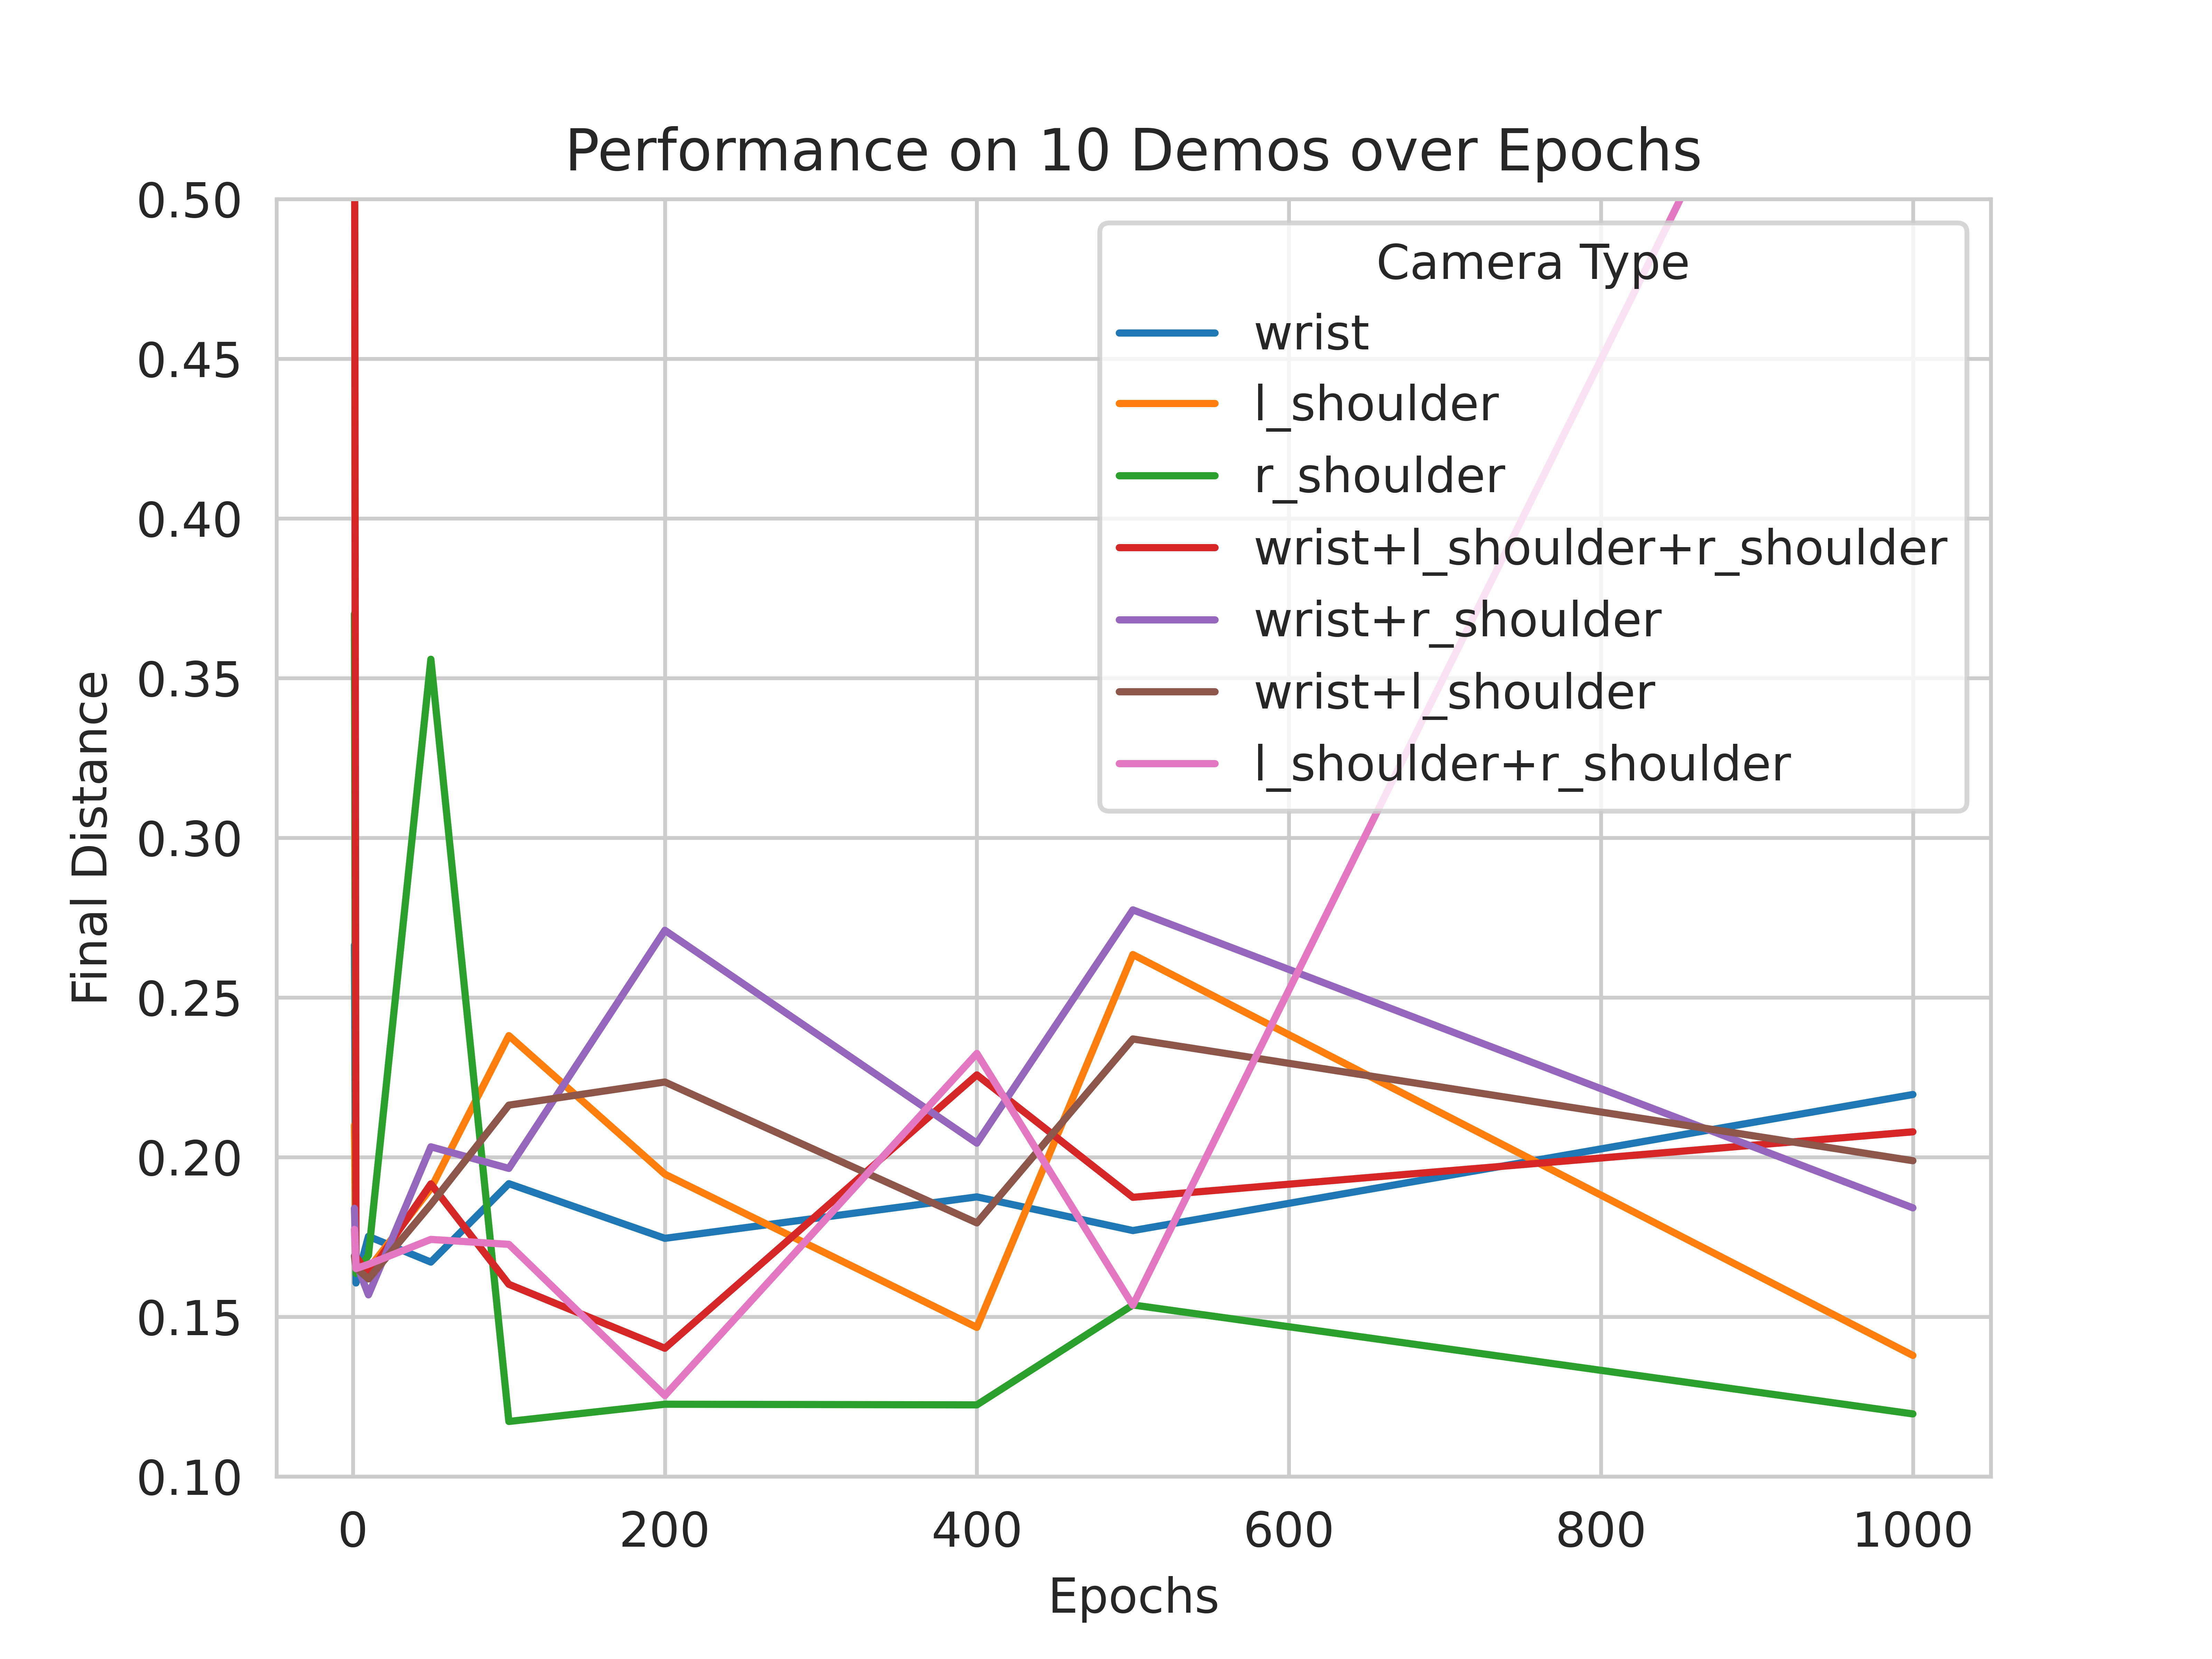
\includegraphics[width=\linewidth]{assets/cam-comb/reach-no-obs/rno_random-cams.png}
    \caption{Average Final Distance to Target}\label{subfig:rno-random-cams-dist}
  \end{subfigure}
  \hfill
  \begin{subfigure}{0.45\linewidth}
    \centering
    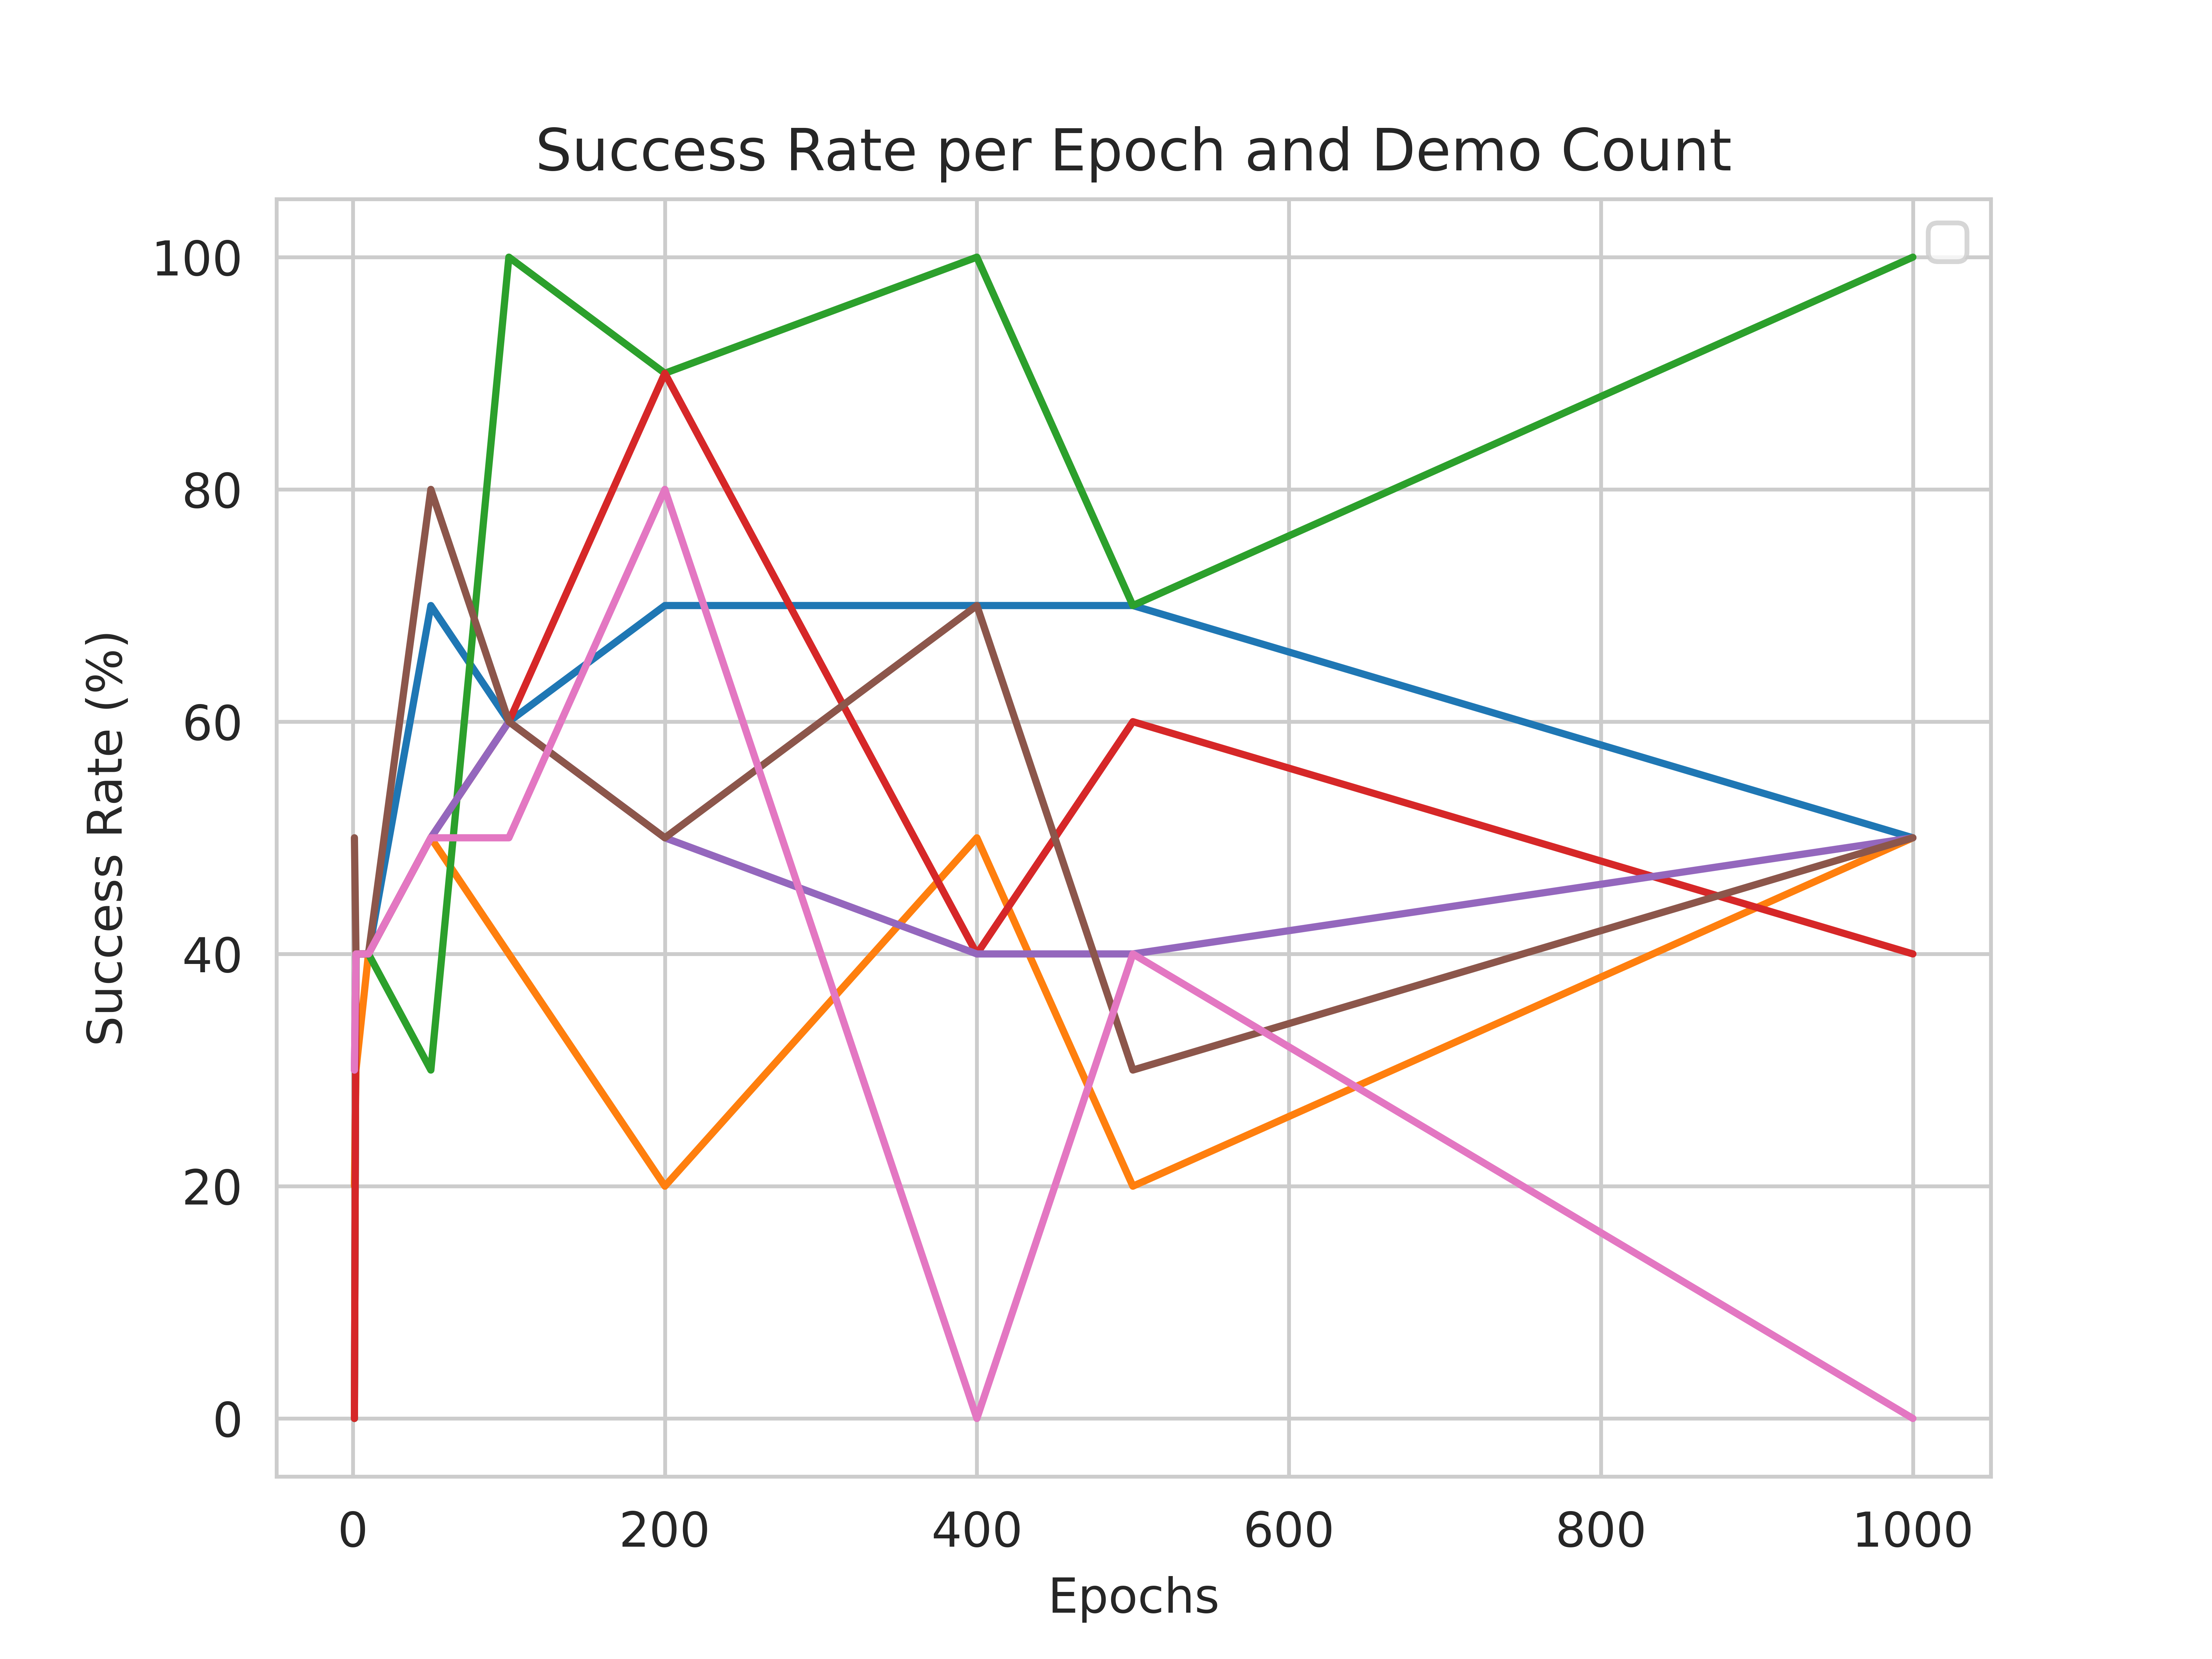
\includegraphics[width=\linewidth]{assets/cam-comb/reach-no-obs/rno_random-cam_success.png}
    \caption{Success Rate (\%) on the $10$ tests}\label{subfig:rno-random-cams-success}
  \end{subfigure}
  \caption{Experimenting with multiple RGB cameras}\label{fig:rno-random-cams}
\end{figure}

\subsection{Increasing the Toy Task Complexity}
Complexity of tasks can be increased in two main ways:
\begin{enumerate}
  \item Increase the movement or the level of interaction of the task at hand
  \item Introducing non-linearities to the environment to make a scene more challenging to traverse for an agent
\end{enumerate}
I plan to do these mainly by introducing obstacles; which will guide me to understand what an agent needs to understand navigation. Secondly, I want to branch out to a grasping task, to increase the number of items of execution, to evaluate the capability of an agent to use its understanding to complete increasingly more complicated tasks.\todo[color=green]{clean up depending on the chosen order}


% Grasping tasks
\section{Expanding the Task Space: Grasping Tasks}
Another task which is likely to suffer from lack of viewpoints is a grasping task. I first designed
a simple version (Figure \ref{fig:grasp-simple}) which the agent learns to reach then grasp the cubic target. 

Main differences between this and the reaching task is that the target here is tangible, so on top of being rendered it is also set to be \emph{collidable}. Another major addition is the usage of the \emph{extension string} as seen in \ref{subfig:simple-zoom-actions}, this instructs the demonstration engine to insert certain moves within the calculated trajectory. In this case \verb|open_gipper()| ensures the gripper is open, then a later waypoint will instruct it to close. 

As the task complexity increases, its design complexity also increases. Also, without any prior knowledge about 3D simulators and 3D design, it took me quite a long time to hunt everything about CoppeliaSim, RLBench, and PyRep to put these together. One criticism I have on these tools is the documentation is all over the place. \todo[color=green]{too ranty? rewrite or remove}

The more complicated counterpart, shown in Figure \ref{fig:grasp-move}, is a scenario where the cube needs to be picked up then moved to the target location (designated in green).

\begin{figure}[htpb] % htpb allows all placement
  \centering
  \begin{subfigure}{0.3\linewidth}
    \centering
    \includegraphics[scale=0.2]{../fyp/assets/task-pics/grasp/simple-front.png}
    \caption{Front}\label{subfig:simple-front}
  \end{subfigure}
  \hfill
  \begin{subfigure}{0.5\linewidth}
    \centering
    \includegraphics[scale=0.3]{../fyp/assets/task-pics/grasp/simple-front-zoom-gripper_actions.png}
    \caption{Zoomed, with gripper action}\label{subfig:simple-zoom-actions}
  \end{subfigure}
  \caption{Simple Grasping Task}\label{fig:grasp-simple}
\end{figure}

\begin{figure}[htpb] % htpb allows all placement
  \centering
  \begin{subfigure}{0.45\linewidth}
    \centering
    \includegraphics[scale=0.2]{../fyp/assets/task-pics/grasp/move-front.png} 
    \caption{Front}\label{subfig:grasp-move-front}
  \end{subfigure}
  \hfill
  \begin{subfigure}{0.45\linewidth}
    \centering
    \includegraphics[scale=0.2]{../fyp/assets/task-pics/grasp/move-top.png}
    \caption{Top}\label{subfig:grasp-move-top}
  \end{subfigure}
  \caption{Grasping then moving}\label{fig:grasp-move}
\end{figure}\todo[color=blue]{reshape}


\todo{add a picture with the cube grasped and the wrist camera view seen at that point}

Initially the wrist camera shouldn't pose any problems. Although, I suspect as we advance through the task, especially after we have grasped something, wrist camera becoming heavily obstructed will render it unreliable so basing our decisions on this medium alone might not be ideal.


\todo[color=pink]{experiments here, or move this where I can get some data on this}
\subsubsection{Observations}
What I got from these experiments was that the agent can benefit from understanding its surroundings at a higher level, and more importantly remembering them. This is because once thek camera becomes obstructed, as with \textbf{Grasp Then Move}, even if the agent could do some exploration to find the target, it wouldn't be ideal due to the restricted view it has access to. So, observing the environment before, and remembering important parts will be vital for the later stages of tasks. I aim to explore some pre-policy visual exploration of the environment then feed this information forward, possibly when it might be needed. For example residual forwarding of data might be used later \todo{should I keep this here?}


% Reaching (Obs) tasks
\section{Reaching with an Obstacle}
Circling back to reaching, I introduced an obstacle placing mechanism as well as randomly placing the target behind this obstacle, ensuring the agent doesn't learn where exactly target is by looking at just the obstacle\todo[color=purple]. See Figure \ref{fig:reach-obs-random} for how this task looks and the check \todo[color=green]{add appendix link, and code} for the backend wiring of the task.

\subsection{Creating the Task}
There are two versions of this task, I thought it might be interesting to randomise the object firstly dependently then independently on the obstacle. The `dependent' randomisation called \verb|ReachObs_Random| samples the obstacle, which in turn controls the spawn boundary of where the target can spawn in, meaning the target will always appear behind the obstacle albeit, edges of it can sometimes stick out. Conversely, the `independently' random version, called \verb|ReachObs_IndRandom|\todo{also add to appendix and link here}, keeps the target spawn boundary fixed, meaning the target can be anywhere in the visible workspace, but it is not necessarily always covered by the obstacle. I can see that this potentially can be useful to keep the dataset a bit more diverse, and allow the wrist camera initially observe the target sometimes.\todo[color=red]{use this somewhere, or hint back to it, maybe even to say there was no difference}

\begin{figure}[htpb] % htpb allows all placement
  \centering
  \begin{subfigure}{0.3\linewidth}
    \centering
    \includegraphics[scale=0.3]{../fyp/assets/task-pics/reach-obs/random-front.png}
    \caption{Front}
  \end{subfigure}
  \hfill
  \begin{subfigure}{0.3\linewidth}
    \centering
    \includegraphics[scale=0.3]{../fyp/assets/task-pics/reach-obs/random-side.png}
    \caption{Side (Left)}
  \end{subfigure}
  \hfill
  \begin{subfigure}{0.3\linewidth}
    \centering
    \includegraphics[scale=0.3]{../fyp/assets/task-pics/reach-obs/random-top.png}
    \caption{Top}
  \end{subfigure}
  \vfill
  \begin{subfigure}{0.45\linewidth}
    \centering
    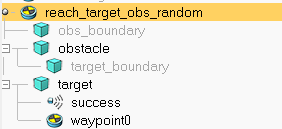
\includegraphics[scale=0.5]{assets/early-work/obs-random-scene-hierarchy.png}
    \caption{`ReachObs\_Random' Scene Hierarchy}
  \end{subfigure}
  \hfill
  \begin{subfigure}{0.45\linewidth}
    \centering
    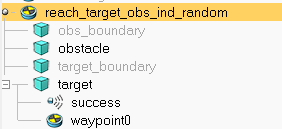
\includegraphics[scale=0.5]{assets/early-work/obs-ind-random-scene-hierarchy.png}
    \caption{`ReachObs\_IndRandom' Scene Hierarchy}
  \end{subfigure}
  \caption{Reaching Task with an Obstacle}\label{fig:reach-obs-random}
\end{figure}\todo[color=blue]{smaller?} 

\subsection{Experiments}\todo[color=red]{not sure what is meant to happen here, maybe move the seq trhing to grasping above and only talk about data here}

\subsubsection{Using same unchanged policy form ReachNoObs}
Unsurprisingly this did not perform very well, 
\begin{figure}[htpb] % htpb allows all placement
  \centering
  \begin{subfigure}{0.45\linewidth}
    \centering
    \includegraphics[width=\linewidth]{assets/cam-comb/reach-obs/ro_random-dist-20demos.png}
    \caption{}\label{subfig:ro-random-dist20}
  \end{subfigure}
  \begin{subfigure}{0.45\linewidth}
    \centering
    \includegraphics[width=\linewidth]{assets/cam-comb/reach-obs/ro_random-success-20demos.png}
    \caption{}\label{subfig:ro-random-success-20}
  \end{subfigure}
  \caption{}\label{fig:ro-random-cams}
\end{figure}

\subsubsection{Understanding the Data Management}
I had initially designed the system to flatten the given demonstrations and then draw from them during the training. However, one drawback with this is that we cannot incorporate any shuffling in the data. \todo

\todo{mention switching to demo dataset}
\missingfigure{shuffling plots, might not add this at all to the report, to be confirmed}
Talk about how the data is loaded and created and managed for the network, talk about shuffling mechanisms and what I've found etc. talk about \verb|shuffle_obs_in_demo| and the other one.

\subsection{Improvements}



\subsubsection{Wrist Camera Alone isn't Enough}
As expected this is where the single wrist camera started showing its shortcomings. The agent would easily move around the obstacle, however, would struggle to make the last steps in touching the target. This is mostly due to the fact that the demonstrations (which are provided by RLBench) are not necessarily pointing the wrist of the robot and hence the camera mounted there to look towards the target. This means that the behavioural cloning agent learns to to the swaying motion around a large grey body, however, is not aware of the obstacle, or even understand the task is related to reaching for the obstacle and depends on its visual cues. 

\todo{add graph of going around the obstacle but not quite reaching the target (wrist)}
\todo{show this with other combinations of cameras, comment on if the l/r without wrist can learn to go around the obstacle easily? maybe not, generalisation might be hard with no wrist}

From experiments I have realised that it learns to move around the obstacle easily, using simple behavioural cloning. However, getting the last nudge to actually reach the target is where it falls apart, especially in more realistic scenarios where the target is randomised behind the obstacle. For static placement behind the wall, the agent, expectedly is quite good. \todo{maybe explain or evidence this, plateaus aroudn the same distance value and watchig t heroot act comfirms this}

\subsubsection{Other Cameras}\todo{rename}
So, we can confirm that the wrist camera alone is not sufficient \todo{ref}, and the combination of wrist and other cameras are almost always better as more coverage of the workspace guarantees less occlusions and more information the agent can work with to make decisions. It was clear that the wrist camera alone wasn't going to cut it unless it learnt to look towards the target, so that inherently some target understanding can be encoded into a task.\todo[color=red]{looking at he target??}


\todo{talk about the policy using differnt camera inputs to blend and make informed choices? maybe some plots here showing if it is better or not?}

\todo{this is important for plan2 later, as that would depend on such a mechanism, hint and even link that from here}

\subsubsection{Implementing `Looking' into the Demonstrations}\todo{haven't done this yet}\label{ew-looking-at-target}
issues this is not easy might be working on this as a part of approach 2 later
Another solution might be to experiment with the demonstration system to make sure we are pointing the wrist camera (so, the hand of our robot) towards its target as a demonstration trajectory is calculated \todo{explain that this proved tricky and might not even be worth it}

If we can't implicitly encode the `looking' information through the demonstration that means we will have to inject this information into our agent some other way. Another way to make sure agent understands to look at the target is teaching it to actively seek out its target, either following previous works such as \todo{find some prior info tracking works add ref} where object priors are incorporated into the learning or with attention mechanisms that figure out what is important in a task without prior object information \todo{maybe reference this later}.  

\subsection{Attending on a Camera in Given Combination}
One of the first ideas, that was bordering on `active vision' was to selectively accept the encoding from a single camera depending on what it was seeing. 


\todo{talk about the implementation of the }
\subsubsection{MultiCNN}
\todo{explaint the implementations, maybe connect to }
\subsubsection{SingleCNN}
I initially though to disconnect the convolutional network, thinking the information can be encoded per view and then fused together to assign better meaning to the given pose. However, with the same logic the scene is still the same scene and encoding features together means that the network will learn to \todo{find a nice way to say the network will learn its fusing in the conv layers. maybe make sure it can}

% Depth Interfacing - under grasping
\section{Depth Interfacing}
Another area of important research, before relating all this back to active vision, is figuring out distance. Depth interfacing is an important part of perception. Continuing from the drawn parallels to humans, we place object in our fields of vision by our two eyes. Stereo-vision, allows us to process two slightly different poses of a target object to reinforce our understanding of where that object is in the environment around us. Other information such as lighting (and shadows) may unconsciously help us as well. The main takeaway is that understanding distance to an object goes a long way in firstly understanding how to approach an object.

There are a few ways to achieve this in robotics. In RLBench specifically is either to use two cameras (with a known distance between the two cameras to adjust poses with known intrinsics). However, RGB cameras are not the only things we have access to. We also we have a depth sensor.

This is because, as I hinted earlier in the background section, the main idea of active vision is to be able to use minimal amounts of viewpoints and make the most out of these. In this scenario, I want to see if it can be justified to use the wrist camera accompanied by the wrist depth sensor to replace any other cameras we might have around the workspace. Paving the way to the next section in proposing active vision policies that act solely on information from a repositionable sensor.

Therefore, it is important to study shortcomings of individual sensors with respect to others to understand how policies with limited access to sensors can be made to overcome such challenges without necessarily adding more points of observability to a workspace.

\subsection{Grasping with Varying Depths}
To start investigating, I devised the following test task to see how the agent reacts to differently sized targets that might be placed at varying distances from the gripper within the scene

\subsubsection{Task Design}
A grasping task makes sense for this experiment. Because unlike the reaching tasks from earlier, the robot will need slightly more precision in executing its grasp and actually grabbing the target. The task performer needs to figure out where an object is before attempting to grab it. So, I created a modified version of the simple grasping task where the target object's distance and scale can be externally varied to observe the behaviours of agents in a controlled manner.\todo[color=green]{talk about delegating the task creating and param passing as well as the tasks in appendix and link here}

\begin{figure}[htpb] % htpb allows all placement
  \centering
  \begin{subfigure}{0.4\linewidth}
    \centering
    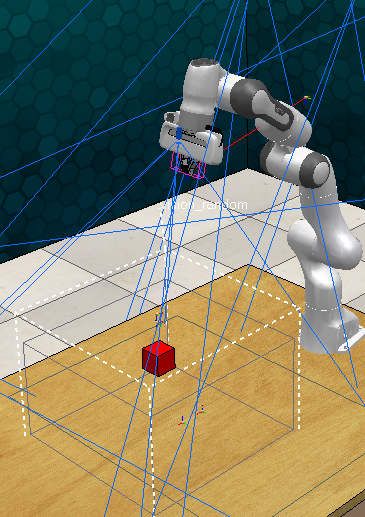
\includegraphics[width=0.7\linewidth]{assets/depth-interfacing/normal-size-grasp.png}
    \caption{Normal Target Size}\label{subfig:normal-grasp}
  \end{subfigure}
  \begin{subfigure}{0.4\linewidth}
    \centering
    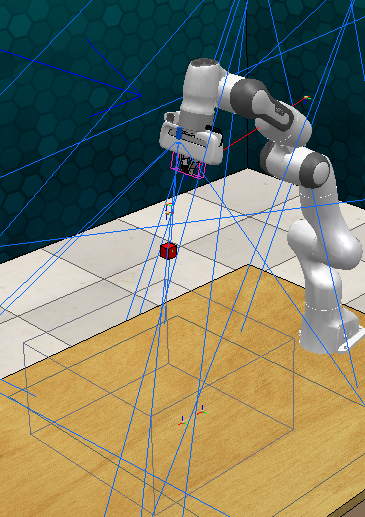
\includegraphics[width=0.7\linewidth]{assets/depth-interfacing/smaller-grasp.png}
    \caption{Smaller Target Size}\label{subfig:small-grasp}
  \end{subfigure}
  \caption{Visualisation of the Depth Interfacing experiment task}\label{fig:di-task}
\end{figure}

Figure \ref{fig:di-task}, is the general setup I am planning on using to evaluate the depth sensor versus a multi-view setup. Initial observations from the side clearly indicate that these are two different targets and will require different reach lengths before the agent can attempt to grab them.

\begin{figure}[htpb] % htpb allows all placement
  \centering
  \begin{subfigure}{0.4\linewidth}
    \centering
    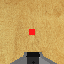
\includegraphics[width=0.7\linewidth]{assets/depth-interfacing/normal-size-wrist.png}
    \caption{Smaller - Wrist RGB}\label{subfig:normal-rgb}
  \end{subfigure}
  \begin{subfigure}{0.4\linewidth}
    \centering
    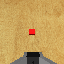
\includegraphics[width=0.7\linewidth]{assets/depth-interfacing/smaller-wrist.png}
    \caption{Smaller - Wrist RGB}\label{subfig:small-rgb}
  \end{subfigure}
  \begin{subfigure}{0.40\linewidth}
    \centering
    
\includegraphics[width=0.7\linewidth]{assets/depth-interfacing/normal-depth.png}
    \caption{Wrist Depth Mask - Normal}\label{subfig:normal-depth}
  \end{subfigure}
  \begin{subfigure}{0.40\linewidth}
    \centering
    
\includegraphics[width=0.7\linewidth]{assets/depth-interfacing/smaller-depth.png}
    \caption{Wrist Depth Mask - Smaller}\label{subfig:small-depth}
  \end{subfigure}
  \caption{Wrist RGB and Depth Masks for the tasks}\label{fig:di-rgb-vs-depth}
\end{figure}

However, as seen in the comparison in \ref{subfig:normal-rgb} and \ref{subfig:small-rgb}, the RGB outputs look practically the same, and will very likely produce extremely similar features after extraction. A way to differentiate them would be to utilise the wrist depth mask in this encoding. As shown in \ref{subfig:normal-depth} and \ref{subfig:small-depth}, they now carry different features in those areas. In the depth mask the darker colours indicate closer objects, and the information is encoded as floats. 

\begin{figure}[htpb] % htpb allows all placement
  \centering
  \begin{subfigure}{0.40\linewidth}
    \centering
    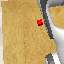
\includegraphics[width=0.7\linewidth]{assets/depth-interfacing/normal-l_rgb.png}
    \caption{Normal - Left Shoulder RGB}\label{subfig:normal-l-shoulder}
  \end{subfigure}
  \begin{subfigure}{0.40\linewidth}
    \centering
    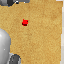
\includegraphics[width=0.7\linewidth]{assets/depth-interfacing/normal-r_rgb.png}
    \caption{Normal - Right Shoulder RGB}\label{subfig:normal-r-shoulder}
  \end{subfigure}
  \begin{subfigure}{0.40\linewidth}
    \centering
    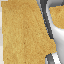
\includegraphics[width=0.7\linewidth]{assets/depth-interfacing/smaller-l_rgb.png}
    \caption{Smaller - Left Shoulder RGB}\label{subfig:smaller-l-shoulder}
  \end{subfigure}
  \begin{subfigure}{0.40\linewidth}
    \centering
    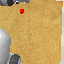
\includegraphics[width=0.7\linewidth]{assets/depth-interfacing/smaller-r_rgb.png}
    \caption{Smaller - Right Shoulder RGB}\label{subfig:smaller-r-shoulder}
  \end{subfigure}
  \caption{Left and Right Shoulder RGB Cameras}\label{fig:di-lr-shoulder}
\end{figure}


Another possible differentiating factor, and the reason earlier tasks were performing well, is due to the shoulder cameras. These also provide extra information about the scene the agent can use to understand its 3D geometry, even if it isn't explicitly taught. Although these are also not perfect, as seen in \ref{subfig:smaller-l-shoulder}, this camera is completely obstructed by the robot and is not seeing the target. This is not immediately problematic, because a smart enough system might be able to reason that the target is visible on the right and not on the left, leading to devising the correct depth for it. However, I have not intentionally encoded that information and doubt this network will be able to produce correct results with these observations.

\subsubsection{Adding Stereo Wrist Vision}\todo[color=blue]{can be removed not sure}
A possibility to overcome this \emph{self-occlusion} is to introduce stereo vision at the wrist level. Adding 2 off-centre cameras to the gripper, likely to the left and right of the existing wrist camera, will fix the self-occlusion, and possibly create a better comparison to the \emph{Wrist RGB} and \emph{Wrist Depth} combination. However, this comes with a lot of rewiring of RLBench and with its likely hidden issues that will pop up later. I did not want to take on this large architectural change before continuing with main investigation of the project, however, if timings permit this will be an important addition to the testing suite.

% proposed policies and learnings
\section{Multi-View Understanding Policies}
On top of just naively combining cameras and expecting the policy to understand what it means to `see' is a tall order. The next step is to understand how we can make the most of the information we are given by incorporating the various views and sensors and seeing what combination makes the most sense.

\subsection{Feature Extraction}
So far, I have been using a simple CNN and extracting 

\subsubsection{Better Feature Understanding}


\subsubsection{Simple Stacking}
This is the naive method of just stacking the view information, which is what I have been using up until this point. Simply stacking information on the channel dimension and feeding them into the network. This has clear disadvantages. Firstly, for the RGB cameras, there is definite misalignment, all these cameras have different poses and will disagree on what they see. This will lead to features not lining up leaving us with an non-optimal and more importantly a brittle policy. Meaning slight variations might confuse and move the policy out of distribution.

\subsection{Fusion}
The other level up is fusion of features. The CNNs used can be expanded 
\subsubsection{Late Fusion}

\subsubsection{Mid-Level Fusion}
Have I ever done something on this?? not really maybe talk about how imma use the shoulder stuff with this,


This adds onto before, gated attention and rgb attending to depth etc, explain some approaches

\subsection{Deeper/Better Feature Understanding - RCNN}
Another thing I wanted to try was to include off-the-shelf models to help extract features and information from my views. As one of the problems I described faced earlier was from the agent not remembering the earlier information that it has seen, I believed an important part of increasing the workspace understanding would be to incorporate residual connections.

I experimented with various sizes of ResNet networks \todo[color=green]{reference}. I essentially replaced my own \verb|CNNEncoder| block with modified versions of \emph{resnet18, resnet34, and resnet50} \todo[color=green]{maybe not mention all, afterall the large ones will be ass when the image is so small}. I had to modify these, because the unmodified version using a main CNN of kernel size $7$ was too large and appropriate features were not being extracted from the views I was feeding. This was evident from observing the agent act in a test scenario where the arm would do nothing remotely similar to what the demo did, or even what the task is about.\todo{maybe a picture of the arm doing some bs here}. \todo[color=pink]{run the original confirm it does not work, if not get a diagram of kernel sizes 7 and 3 and an explanation why this might be the case.}

The modified versions, with a smaller kernel, feeding into the later layers and then getting the residual connection didn't seem to work any better either \todo[color=pink]{test on comparing my one with a resnet graph on a toy grasping task, maybe grasp then move?}

A reason these might not have worked well is because of one of my earlier constraints. The image sizes being \(64 \times 64\) pixels, might not be enough to extract meaningful information with a ResNet. This is likely due to its aggressive pooling between the layers and especially during the residual connection and the aggressiveness only increases in larger models. \todo[color=red]{not actually sure if this is right, fact check, wrote this some time ago} 

\subsubsection{increasing the camera view for experimentation}\todo[color=red]{larger image trials? expand the task to be lager 128 or even 224 seems common with resnet}

\subsection{Temporal Understanding of Demonstrations}
Even though the agent is not half bad at trying to reach the target in the above configurations, it is not necessarily better at succeeding at grasping, and the movements seem janky compared to the  precise demonstrations given. I believe this is because the robot is only given its current view and does not understand where it might be during the epsiode \todo{this is the issue I faced}

and the robot doesn't necessarily understand where in the movement it is, because the first half of the episode is very repetitive and the inputs are eerily similar. This meant that an important part of the system was for my agent to understand where it was as well as when it was.

\subsubsection{Latent RNN Encodings of Movement Steps}
I wanted to encode the timestep information into some sort of feature representation which would use the previous states to encode the data. This simple idea was to introduce temporal noise into the decision process. Then act on the final encoding


\missingfigure{diagram about feeding the entire demo and training per step}

\todo{problems here were that the entire demo was being used, but the optimisation was getting made at the final state}

\subsubsection{Fine-Grained per Time-Step Training}
Once I realised my mistake, which was about discarding half my encoded steps and were not using my RNN to its full potential \todo{rewrite} As I have access to ground truth information at every observation step, it would be smart to optimise the loss in a fine-grained manner at every frame.
\missingfigure{updated diagram to convey the padding and unpacking and training the loss on every frame step}
This lead to a more robust and confident architecture. The movements of my policy felt less spiky, no more sudden jerks and more calculated reaching. It did still absolutely overfit to the average position, and was not much better at grasping, but the episodic movements were cleaner and I believe enhancing the grasping branch of the network would allow it to be more successful \todo{what the fuck am i talking about, summarise and clean up}


\subsection{ViT Encodings}
\todo[color=red]{not done much on this, but may be able to talk about how I would go about it or just remove}

\section{Proprioception}\todo{maybe talk about why I left it out earlier in the chapter}
Up until this point, I left proprioceptive data out of the training, mainly because I wanted to train on purely visual feedback to see what it could achieve without any other state information. Secondly, including state information about the robot, would not necessarily immediately help with the 

\section{Moving to \emph{Active Vision}}


\todo{improve the grasping}

\todo{It might be worth scaling everthing to 128 by 128 next week and do a repeat run so that I can at least say that I have done it}

\todo{ruun grasp then move and confirm the suspicions of the policies with no memory failing.}


